% !TEX root = ../main.tex

%************************************************
\chapter{Introduction}
\label{ch:intro}
%************************************************

The first quasar was discovered when it was found that the star-like, thirteenth magnitude objected associated with the radio source 3C 273 was at a cosmological distance \citep[$z=0.158$;][]{schmidt63}. 
This implied an enormous luminosity ($4\times10^{12}$L$_\odot$) for such a compact source and it was quickly realised that energy source was the release of gravitational potential energy as mass is accreted onto a supermassive black hole at the centre of a galaxy \citep[e.g.][]{hoyle63,salpeter64,lynden-bell69,lynden-bell71}. 
\marginpar{Super-massive: $10^{6 - 9}$ M$_\odot$}

\section{The AGN-host galaxy connection}

Super-massive black holes (BHs) are found at the centres of most nearby massive galaxies \citep[e.g.][]{kormendy95,ferrarese05,kormendy13}.
Remarkably, given their spatial scales differ by many orders of magnitude, the BH mass and mass of the host galaxy spheroid are strongly correlated \citep{ferrarese00,gebhardt00,graham01,tremaine02,marconi03,aller07,gultekin09}.  
Although any underlying causal mechanism(s) responsible for the correlation is yet to be conclusively identified, there is considerable observational and theoretical support for a `feedback' relationship in which the energy output from rapidly accreting BHs (in a quasar phase) couples with the gas in the host galaxy and quenches star formation \citep[e.g.][]{silk98,king03,dimatteo05,king15}. 

Quasar feedback has also been invoked to explain the similarity of the cosmic BH accretion and star formation histories.
The number density of quasars, which evolves strongly with redshift, peaks at redshifts $2 \lesssim z \lesssim 3$ \citep[e.g.][]{brandt05,richards06b} and the most massive (M$_\bullet \gtrsim 10^9\msun$) present-day BHs experienced much of their growth during this epoch.  
The star formation rate, which closely follows the cosmological evolution of the quasar luminosity function, also peaks during this epoch \citep[e.g.][]{boyle98}. 
Quantifying the growth-rate of massive BHs at $2 \lesssim z \lesssim 3$ would therefore help significantly in understanding the role quasars play in galaxy evolution.

\section{Measuring black hole masses}

As one of just two fundamental quantities describing a BH on astrophysical scales, the mass is of crucial importance to virtually all areas of quasar science, including the evolution and phenomenology of quasars, and accretion physics.
The power output of quasars is directly proportional to the BH mass. 
There is much debate regarding what effect the energy output by quasars has on evolution and structure of the host galaxy. 

The masses of BHs in many local, inactive galaxies have been measured by dynamical modelling spatially resolved kinematics. 
However, this requires the sphere-of-influence of the BH, $R_{\rm BH}$, to be resolved. 
\marginpar{$R_{\rm BH} = \frac{2GM_{\rm BH}}{\sigma\ast}$} 
With masses only $\sim$0.1 per cent of the stellar masses of the host galaxies, $R_{\rm BH}\sim1-100$ pc.
With current instrumentation, resolving this region is only possible in very close by, inactive galaxies. 

The reverberation mapping method, first proposed by \citet{blanford82}, uses the time delay between continuum variations and emission-line variations to estimate the size of the BLR. 
Because it depends on time resolution rather than spatial resolution, it can applied out to much greater distances. 
This means that 

\subsection{Reverberation mapping}

Material is pulled towards the SMBH at the centre and sheds angular momentum through viscous and turbulent processes in an accretion disk, which radiates primarily at ultraviolet (UV) to soft-X-ray wavelengths. 
Strong optical and UV emission lines are produced in photo-ionised gas clouds moving rapidly around the BH at distances from several light-days to several light-months.
The Doppler-broadened emission line widths imply gas cloud velocities of thousands of km s$^{-1}$ in this {\it broad-emission line}. 

Continuum variability is a common characteristic of quasars. 
Because the BLR is photo-ionized by the continuum, the broad emission lines also vary with some characteristic lag, which is related to the light travel time across the BLR. 
The reverberation mapping technique uses the time lag between variations in the continuum emission and correlated variations in the broad line emission to measure the typical size of the BLR. 
Today RM has become a practical and powerful tool to study BLRs (see reviews by, e.g., Peterson 1993; Netzer \& Peterson 1997; Horne et al. 2004). 

Under the assumptions that the BLR dynamics are virialised and the gravitational potential is dominated by the BH, the BH mass is simply given by the product of the typical BLR radius and the square of the virial velocity of the BLR clouds. 
In practice, reverberation mapping relies on dense spectrophotometric monitoring campaigns which span many years. 
The typical velocity in he BLR is measured from the width of he broad \hb lines in the RMS spectra, ensuring that only the variable part of the line contributes to the line width calculation. 
Since the structure and geometry of the BLR is unknown, a virial coefficient $f$ is introduced to transform the observed line-of-sight velocity inferred from the line width in to a virial velocity. 
In practice, the value of is empirically determined by requiring that the derived masses are consistent with those predicted from the M-$\sigma$ relation for local inactive galaxies. 
Although this technique has proved to be effective, because it relies on resource-intensive spectro-photometric monitoring campaigns, masses have been derived for only $\sim50$ AGN, all at low redshifts $z\lesssim0.3$. 
There are now several dozens of AGNs and quasars (most are at redshifts $z<0.3$) with average lag measurements \citep[e.g.][]{kaspi00,peterson04,bentz09,denney10,barth11,grier12}. 
The current sample is strongly biased toward relatively low-luminosity AGNs, mostly nearby Seyfert 1 galaxies.
A number of Palomar-Green (Schmidt \& Green 1983) quasars are included, but the highest-redshift
source studied is only at z = 0.29 (PG 1700+518).
The uncertainty in the reverberation-mapping masses is $\sim0.4-0.5$ dex \citep[e.g.][]{peterson10}.

If the line-emitting clouds in the broad line region (BLR) are assumed to be virialised and moving in a potential dominated by the central BH, then the BH mass is simply a product of the BLR size and the square of the virial velocity (give equation)
The reverberation-mapping technique uses the time lag between variations in the continuum emission and correlated variations in the broad line emission to measure the typical size of the BLR \citep{peterson93,peterson14}. 
The full width at half maximum (FWHM) or dispersion ($\sigma$; derived from the second moment) velocity of the prominent broad emission line of \hb (4862.7\AA)\footnote{Vacuum wavelengths are employed throughout the thesis.} 
is used as an indicator of the virial velocity, with extensions to other low-ionization emission lines such as \ha (6564.6\AA) and \ion{Mg}{II}\ll2796.4,2803.5 \citep[e.g.][]{vestergaard02,mclure02,wu04,kollmeier06,onken08,wang09,rafiee11}.
\marginpar{FWHM: Full width of the line profile at half of maximum intensity}
Extensive reverberation mapping campaigns have provided accurate BH masses for $\sim$50 active galactic nuclei (AGN) at relatively low redshifts and of modest luminosity \citep[e.g.][]{kaspi00,kaspi07,peterson04,bentz09,denney10}. 

\subsection{Single-epoch virial estimates}

Single-epoch virial BH mass estimates normally take the form

\begin{equation}
  \label{eq:virialmass}
  \mathrm{M_{BH}} = 10^{a} \left( \frac{\Delta V}{1000~\mathrm{km~s^{-1}}} \right)^b \left[ \frac{L_{\lambda}}{10^{44}~\mathrm{erg~s^{-1}}} \right]^c
\end{equation}

\noindent where $\Delta V$ is a measure of the line width (from either the FWHM or dispersion), $L_\lambda$ is the monochromatic continuum luminosity at wavelength $\lambda$, and $a$, $b$, and $c$ are coefficients, determined via calibration against a sample of AGN with reverberation-mapping BH mass estimates. Several calibrations have been derived using different lines (e.g. \hbns, \ion{Mg}{II}, \ion{C}{IV}) and different measures of the line width (FWHM or dispersion) \citep[e.g.][]{vestergaard02,mclure02,vestergaard06,mcgill08,wang09,rafiee11,park13}.

Reverberation mapping campaigns have also revealed a tight relationship between the radius of the BLR and the quasar optical (or ultraviolet) luminosity \citep[the $R-L$ relation; e.g.][]{kaspi00,kaspi07}.
The emission-line spectrum from an ionized gas, setting aside elemental abundances,
is largely controlled by the particle density n and an ionization parameter

\begin{equation}
U = \frac{Q(H)}{4{\pi}R^2nc}
\end{equation}

where Q(H) is the number of hydrogen-ionizing photons emitted per second by the central
object. To some low order of approximation (principally ignoring the Baldwin Effect), all
AGN spectra have similar emission-line flux ratios and similar emission-line equivalent
widths, suggesting that U and n do not vary much from one source to another. If we
further assume that Q(H)$\propto$ L where L is the luminosity of the central source in some
arbitrary band, we are led to the naive prediction that R $\propto$ L1/2 .

An advantage of the technique is that it is inexpensive in telescope time. A single spectrum yields a mass measurement. 
This relation provides a much less expensive method of measuring the BLR radius, and large-scale studies of AGN and quasar demographics have thus become possible through the calibration of single-epoch virial-mass estimators using the reverberation-derived BH masses \citep[e.g.][]{greene05b,vestergaard06,vestergaard09,shen11,shen12,trakhtenbrot12}.
The uncertainties in reverberation mapped BH masses are estimated to be $\sim 0.4$ dex \citep[e.g.][]{peterson10}, and the uncertainties in virial masses are similar \citep[e.g.][]{vestergaard06}.
Since the structure and geometry of the BLR is unknown, a virial coefficient $f$ is introduced to transform the observed line-of-sight velocity inferred from the line width in to a virial velocity.
This simplification accounts for a significant part of the uncertainty in virial BH masses \citep[in addition to, for example, describing the BLR with a single radius $R$ and scatter in the $R-L$ relation;][]{shen13}. 
By far the biggest uncertainty is the virial coefficient f . 
It is unknown, and it probably varies from source to source.
A spherical distribution of clouds on random, isotropic orbits has f = 3/4 for $\Delta$V = FWHM and
f = 3 for $\Delta$V = $\sigma$ (Netzer 1990).
Furthermore, if the BLR is anisotropic \citep[for example, in a flattened disk; e.g.][]{jarvis06} then the line width will be orientation-dependent \citep[e.g.][]{runnoe13b,shen14,brotherton15}. 

For example, single epoch estimates have been used to calculate black hole masses in the highest redshift quasars to study the growth of SMBHs. 
This figure shows a compilation of SE mass estimates for quasars over a wide redshift range from different studies. 
These studies show that massive, $10^9$ BHs are probably already in place by $z\sim7$, when the age of the Universe is less than 1 Gyr.
The fact that a SMBH exists in a quasar at such high redshift is of great importance in physics.
The high redshift means that it was already there when our universe was very young, only about
800 million years old. And the fact that a SMBH was able to grow up in such a short time put
some very tight constraints upon both the cosmological parameters and the accretion history of the
SMBH itself (Willott et al. 2003).

Single epoch masses have also been used to study the distribution of quasars in the BH mass-luminosity plane, which conveys important information about the accretion process of these active black holes (e.g. Kollmeier et al. 2016). 
Redshift evolution of BH-bulge scaling relations (e.g. Bennert et al. 2011). 
Clustering (Shen \& Ho 2014; Timins et al.?). 
With the R–L relationship, we are able to explore the black hole mass function, not only locally but at high redshift, enabling us to trace the history of black hole growth.
Some exploratory work has been done on this and in fact there are claims that the M-sigma relation evolves over time. 

We emphasize that application of single-epoch spectroscopy to quasars rests on the untested assumption that machinery which is calibrated for sub-Eddington BHs with M$\sim10^7$ still works for BHs with masses up to $10^{10}$ that radiate near the Eddington limit. 
Refer forward to problems with \ion{C}{IV} (Chapter 3)


Throughout this thesis we adopt a $\Lambda$CDM cosmology with $h_0=0.71$, $\Omega_M=0.27$, and $\Omega_\Lambda=0.73$. 
All wavelengths and equivalent width measurements are given in the quasar rest-frame, and all emission line wavelengths are given as measured in vacuum.

\section{Basic properties}

\begin{figure}
  \centering
  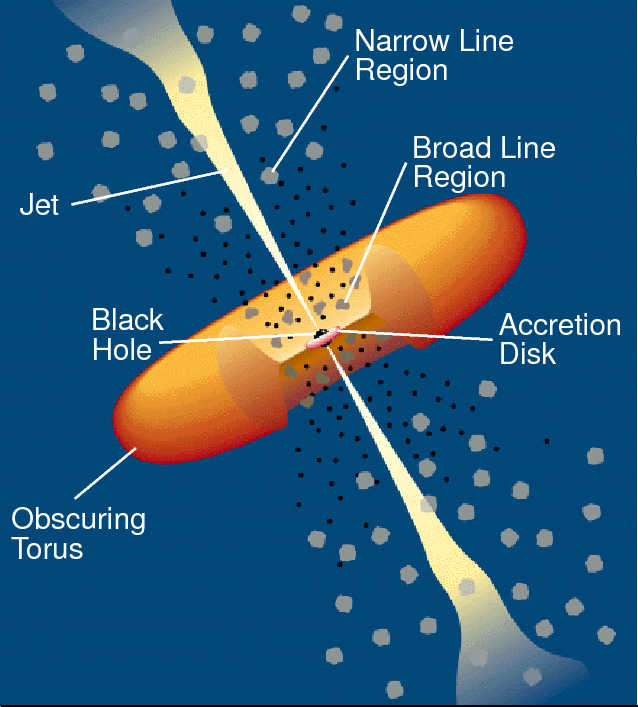
\includegraphics[width=0.5\textwidth]{figures/chapter05/urry_model}
  \caption[{Illustration of the physical structure of an AGN in a simple orientation-based unification model.}]{Illustration of the physical structure of an AGN in a simple orientation-based unification model. Figure taken from \citet{urry95}.}
  \label{fig:agnmodel}
\end{figure}

Unification models attempt to explain all further observational differences as being apparent differences due to {\it orientation} effects. 
The basic physical structure of an AGN in this model is illustrated in Figure \ref{fig:agnmodel}. 

Further away from the central black hole and beyond the dusty torus are slower moving clouds of gas which are photo-ionised by the continuum emission from the accretion disk and produce forbidden emission lines of narrower widths (typically hundreds of km s$^{-1}$). 
Outflows of energetic particles occur along the poles of the accretion disk and form collimated radio-emitting jets and in some cases giant radio-emitting lobes. 

\section{The Torus}

It’s generally believed that the IR emission of an AGN is coming from the dust torus, which
locates at a distance larger than the RBLR. 
Further out are dusty, molecular clouds, the geometry of which is often modelled as a torus co-planar with the accretion disk. 
Along some lines of sight from the observer to the accretion disk / broad line region the dusty torus obscures the UV/optical radiation. 
In this case, an observer would see a weak UV/optical continua and no broad emission lines and classify the AGN as being {\it Type II}. 
On the other hand, if the line of sight is un-obscured by the dusty torus then a broad emission line component would be observable in the spectrum and the AGN would be classified as being {\it Type I}. 

Elitzur \& Shlosman (2006): 

Recent high-resolution IR observations indicate that the torus size might be no more than a few parsecs (Elitzur 2005 and references therein); in particular, VLTI observations of NGC 1068 show that the FWHM size of the 12 mm emission is only 4 pc (Jaffe et al. 2004). 
The compact sizes place the torus inside the region where the SBH gravity dominates over the galactic bulge.

Two approaches have been taken for the torus dynamic origin. 
A hydrostatic scenario depicts the torus as a doughnut-like structure populated by molecular clouds accreted from the galaxy (Krolik \& Begelman 1988). 
However, the origin of vertical motions capable of sustaining the clouds in a hydrostatic structure with H$\sim$R was recognized from the start as problematic and has eluded solution thus far (e.g., Davies et al. 2006). 
The other scenario, based on the seminal work by Blandford \& Payne (1982), involves the outflow of clouds embedded in a hydromagnetic disk wind (Emmering et al. 1992, hereafter EBS92; Konigl \& Kartje 1994; Kartje \& Konigl 1996; Bottorff et al. 1997, 2000; Kartje at al. 1999; Everett 2005). 
In this approach the torus is merely a region in the wind that happens to provide the required toroidal obscuration; i.e., it is that region wherein the clouds are dusty and optically thick.

\section{Outflows and winds}

X-ray and UV spectroscopy has revealed high velocity outflows to be nearly ubiquitous in high accretion rate AGN.
Models of galaxy evolution that invoke AGN feedback require these outflows to reach galactic scales and quench star formation in the AGN host galaxies. 
In recent years, a huge amount of resources have been devoted to searching for observational evidence of these galaxy-wide, AGN-driven outflows. 
This has resulted in recent detections of outflows in AGN-host galaxies using tracers of atomic, molecular, and ionised gas \citep[e.g.][]{nesvadba06,arav08,nesvadba08,moe09,dunn10,alexander10,harrison12,harrison14,nesvadba10,rupke13,veilleux13,nardini15,feruglio10,alatalo11,cimatti13,cicone14}.  

Everett et al. (2005): 

A variety of observational signatures point to the importance of outflowing gas within many types of active galactic nuclei (AGNs). 
Blueshifted absorption features (in broad absorption line quasars, or BALQSOs; see, e.g., Weymann et al. 1991) are seen in approximately 15\% (Reichard et al. 2003) of radio-quiet quasars, with velocities up to 0.1c. In addition, radio-loud quasars display relativistic, collimated outflows. 
There has also been observational evidence that suggests the mass outflow rate in AGNs is nearly equal to the mass inflow rate (see, e.g., Crenshaw et al. 2003; Chartas et al. 2003).

{\it Broad absorption line quasars} (BALQSOs) are a sub-population of quasars exhibiting blue-shifted absorption troughs broader than 2000 \kms \citep{weymann91} which are unambiguously associated with AGN-driven out-flowing gas. 
As well as showing high rates of mergers, an anomalously large fraction of heavily reddened objects exhibit broad blue-shifted absorption troughs in their spectra \citep{urrutia09, glikman12}. 
This observation suggests that the BAL phenomenon may be related to a `blow-out' phase of a quasars lifetime as it transitions from a dusty, obscured objected to a luminous blue quasar, at the same time quenching star formation. 
Since outflows are believed to be fundamental to AGN feedback, a better understanding of their properties could shed light on the outflow phenomenon. 


Throughout this thesis we use the terms `quasar' and `Active Galactic Nucleus (AGN)' interchangeably to refer to all active supermassive black holes, although the term quasar is generally reserved for the luminous (L$_{\rm Bol} > 10^{12}{\rm L}_{\odot}$ subset of AGNs).

\section{Outflows}

X-ray and UV spectroscopy has revealed high velocity outflows to be nearly ubiquitous in high accretion rate AGN.
Models of galaxy evolution that invoke AGN feedback require these outflows to reach galactic scales and quench star formation in the AGN host galaxies. 
In recent years, a huge amount of resources have been devoted to searching for observational evidence of these galaxy-wide, AGN-driven outflows. 
This has resulted in recent detections of outflows in AGN-host galaxies using tracers of atomic, molecular, and ionised gas \citep[e.g.][]{nesvadba06,arav08,nesvadba08,moe09,dunn10,alexander10,harrison12,harrison14,nesvadba10,rupke13,veilleux13,nardini15,feruglio10,alatalo11,cimatti13,cicone14}.  

One particularly successful technique has been observing forbidden emission lines, which trace warm (T$\sim$$10^4$K) ionised gas in the AGN NLR. 
Because of its high equivalent width, [\ion{O}{III}]\l5008 is the most studied of the narrow AGN emission lines. 
In general, the [\ion{O}{III}] emission consists of two distinct components: a narrow, `core' component, with a velocity close to the systemic redshift of the host galaxy, and a broader `wing' component, which is normally blueshifted. 
The general consensus is that the core component traces the gravitational potential of the host galaxy, as the width correlates well with the stellar velocity dispersion. 
On the other hand, the broad, blueshifted wing is tracing outflowing gas. 
This emission appears blueshifted because the far-side of the outflow - that is, the side which is moving away from the line of sight - is obscured \citep[e.g.][]{heckman81,vrtilek85}. 

Observations of broad velocity-widths and blueshifts in narrow emission lines stretch back several decades \citep[e.g.][]{weedman70,stockton76,heckman81,veron81,feldman82,heckman84,vrtilek85,whittle85,boroson92}. 
However, these studies rely on small samples, which are often unrepresentative of the properties of the population. 
More recently, the advent of large optical spectroscopic surveys (e.g. SDSS) have facilitated studies of the NLR in tens of thousands of AGN \citep[e.g.][]{boroson05,greene05a,zhang11,mullaney13,zakamska14,shen14}. 
This has provided constraints on the prevalence and drivers of ionised outflows.   
At the same time, there is strong evidence from spatially resolved spectroscopic observations that these outflows are extended over galaxy scales \citep[e.g.][]{greene09,greene11,hainline13,harrison12,harrison14}. 

However, these studies do not cover the redshift range when star formation and BH accretion peaked, and consequently when feedback is predicted to be strongest. 
At these redshifts the bright optical emission lines are redshifted to near-infrared wavelengths, where observations are much more challenging. 
As a consequence, studies at high redshifts have typically relied on relatively small numbers of objects \citep[e.g.][]{netzer04,sulentic04,shen16a}.
These studies find [\ion{O}{III}] to be broader in more luminous AGN, suggesting that AGN efficiency in driving galaxy-wide outflows increases with luminosity \citep[e.g.][]{netzer04,nesvadba08,kim13,brusa15,carniani15,perna15,bischetti16}. 
The fraction of objects with very weak [\ion{O}{III}] emission alsp appears to increase with redshift and/or luminosity \citep[e.g.][]{netzer04}. 

Other recent studies have looked at the [\ion{O}{III}] emission properties of extreme objects - e.g. heavily obscured quasars \citep{zakamska16} and the most luminous quasars \citep{bischetti16} - at redshifts $z\sim2$. 
The [\ion{O}{III}] emission in these objects is extremely broad and strongly blueshifted. 
These observations are consistent with galaxy formation models that predict AGN feedback to be strongest in luminous, dust-obscured quasars.
 
\section{SEDs}

\ac{AGN} emit strongly over many decades in frequency (Figure~\ref{fig:seyfert_sed}). 
At different frequencies, the emission originates from processes occurring in different regions of the \ac{AGN}. 
Hard X-ray emission is dominated by Compton up-scattering of accretion disk photons by electrons in a hot corona \citep[e.g.][]{sunyaev80}, \ac{UV}/optical by thermal accretion disc emission, \ac{IR} by dust at a wide range of temperatures, and radio by synchrotron emission in relativistic jets.   

Significant diversity is observed in the \ac{SED}s of individual objects. 
However, the systematic study of the dependence of the \ac{SED} shape on physical parameters has, until very recently, been limited by the difficulty in obtaining a large sample of quasars with good multi-wavelength coverage and large dynamic range in luminosity and redshift. 
However, we are able to take advantage of a number of recent, sensitive, wide-field photometric surveys, including SDSS (in the UV/optical), UKIDSS (in the \ac{NIR}) and WISE (in the mid-infrared).
We will combine this information with the \ac{BH} mass and mass-normalised accretion rate estimates and outflow diagnostics which we developed in Chapters~\ref{ch:bhmass} and \ref{ch:nlr}. 
We will determine whether there are \ac{SED}-related systematics as a function of outflow signatures and \ac{BH} mass or Eddington ratio. 

Since the physical processes that power \ac{AGN} are generally understood only qualitatively, almost all \ac{AGN} \ac{SED} templates are empirical. 
The empirical template of \citet{elvis94} is still the most commonly cited, despite many additions and updates \citep[e.g.][]{polletta00, kuraszkiewicz03, risaliti04, richards06,  polletta07, lusso10, shang11, marchese12, trichas12}. 
However, these composite spectra are often constructed from quasars with a huge range in luminosity as a function of wavelength. 
In addition, the presence of significant host galaxy at optical wavelengths in low-redshift objects is an additional complication which has not always been taken care of adequately. 
There is therefore a strong rationale for taking a parametric approach to modelling quasar \ac{SED}s. 
This is the approach we take in this chapter. 


\section{Summary / what I need to get across}

It's a data rich time.
SDSS has been revolutionary - shown the power of large surveys. 
We have wide-field photometry in a number of bands - important because AGN emit strongly over many decades in frequency. 
With spectra from SDSS we can derive BH masses and outflow properties from optical lines. 
But these are shifted to infrared wavelengths at redshifts > 1, when things get interesting. 
Increasing availability of infrared-spectra. 
Looking to the future, huge spectroscopic surveys - WEAVE, 4MOST. 

Quasar black hole masses: \citet{shen13}, \citet{peterson10}, \citet{peterson11}, \citet{vestergaard11}, \citet{marziani12}. 
This has motivated a considerable amount of observational work searching for feedback signatures \citep[for recent reviews, see][]{alexander12,fabian12,heckman14}. 
